\documentclass[preview]{standalone}
\usepackage{amssymb, amsthm}
\usepackage[fleqn]{amsmath}

\usepackage{geometry}
\geometry{paperwidth=12.5cm,margin=0mm}

\usepackage[no-math]{fontspec}
\usepackage{unicode-math}

%\setmainfont{GFS Neohellenic}
%\setmathfont{GFS Neohellenic Math}
%\usepackage{libertinus}
\setsansfont{texgyreheros}[ 
Extension = {.otf}, 
UprightFont = {*-regular}, 
ItalicFont = {*-italic}, 
BoldFont = {*-bold}, 
BoldItalicFont = {*-bolditalic}] 

\usepackage{polyglossia}
\setmainlanguage[babelshorthands=true]{german}
\usepackage[german=guillemets]{csquotes}
\usepackage{microtype}

\usepackage{xcolor}
\definecolor{itwm_blue_04}{RGB}{0,90,148}
\definecolor{background}{RGB}{249,249,249}

\usepackage{tikz}
\usepackage{pgfplots}
\pgfplotsset{compat=newest}
\usetikzlibrary{backgrounds}
\begin{document}
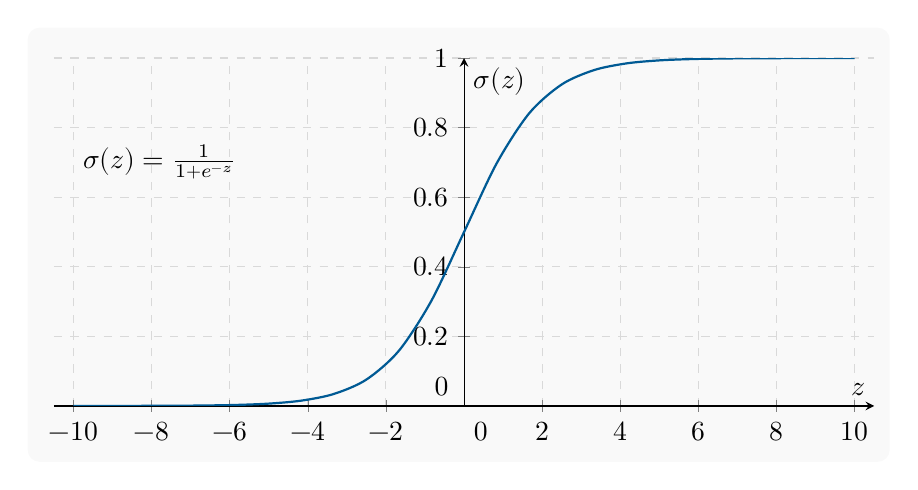
\begin{tikzpicture}[background rectangle/.style=
{fill=background,rounded corners=1ex}, show background rectangle]
\begin{axis}[
    axis lines = center,
    xlabel = {$z$},
    ylabel = {$\sigma(z)$},
    height=6cm, width=12cm, 
    grid=major,
    grid style={dashed, gray!30},
    xmin=-10.5, xmax=10.5, ymin=0, ymax=1.0,  
    xtick = {-10, -8, ..., 10},
    after end axis/.code={
        \path (axis cs:0,0) 
            node [anchor=north west,yshift=-0.075cm] {0}
            node [anchor=south east,xshift=-0.075cm] {0};
    }
]
\addplot[draw=itwm_blue_04, smooth, thick, domain=-10:10]{1/(1+exp(-x)};
\end{axis};
\node [anchor=west] (note) at (0.25,3.1) {$\sigma(z)=\frac{1}{1+e^{-z}}$};
\end{tikzpicture}

\end{document}